\documentclass[12pt, a4paper]{article}

\usepackage[utf8]{inputenc}
\usepackage[T1]{fontenc}
\usepackage[russian]{babel}
\usepackage[oglav,spisok,boldsect,eqwhole,figwhole,hyperref,hyperprint,remarks,greekit]{./style/fn2kursstyle}
\graphicspath{{./style/}{./figures/}}
\usepackage{caption}
\usepackage{subcaption}

\usepackage{multirow}
\usepackage{supertabular}
\usepackage{multicol}


\usepackage{diagbox}
\usepackage{listings}
\usepackage{color}

\definecolor{dkgreen}{rgb}{0,0.6,0}
\definecolor{gray}{rgb}{0.5,0.5,0.5}
\definecolor{mauve}{rgb}{0.58,0,0.82}

\lstset{frame=tb,
	inputencoding=utf8,
	basicstyle=\ttfamily,
	extendedchars=\true,
	showspaces=\false,
	showstringspaces=\false,
	language=Python,
	aboveskip=3mm,
	belowskip=3mm,
	showstringspaces=false,
	columns=flexible,
	basicstyle={\small},
	numbers=left,
	numberstyle=\tiny\color{gray},
	keywordstyle=\color{red},
	commentstyle=\color{dkgreen},
	stringstyle=\color{mauve},
	breaklines=true,
	breakatwhitespace=true,
	tabsize=3
}











\title{Распознавание графиков решения \\ одномерного линейного уравнения переноса}
\author{О.\,Д.~Климов}
\supervisor{М.\,П.~Галанин}
\group{ФН2-61Б}
\date{2024}

\renewcommand{\labelenumi}{\theenumi)}
\begin{document}

\maketitle

\tableofcontents

\newpage

\section-{Введение}
Необходимость распознавания графика функций возникает в совершенно разных прикладных задачах науки и техники. Например, она непосредственно связана с проблемой восстановления графика решений уравнений по неточно заданным данных о решениях. В силу нелинейности распознавания изображений нахождение точных алгоритмов для такой задачи испытывало ряд трудностей. Однако с развитием программирования и вычислительной техники стало возможным решать данную задачу методами нейронных сетей.

\section{Постановка задачи}

\subsection{Формулировка}
Необходимо изучить методы численного решения линейного одномерного уравнения переноса. Составить и отладить программу для нахождения численного решения задачи Коши для указанного уравнения. Использовать шесть различных разностных схем:
\begin{enumerate}
	\item Явная схема с левой разностью на двух точках,
	\item Явная схема с левой разностью на трех точках,
	\item Неявная схема с левой разностью на двух точках,
	\item Неявная схема с левой разностью на трех точках,
	\item Схема Лакса,
	\item Схема Лакса-Вендрофа.
\end{enumerate}
Для всех схем использовать одинаковую систему тестов:
\begin{enumerate}
	\item Левый треугольник,
	\item Правый треугольник,
	\item Прямоугольник,
	\item Косинус,
	\item «Зуб».
\end{enumerate}

Реализовать модель нейронной сети для распознавания решения на языке программирования Python. На основе модели разработать программу, которая по неточному решению возвращает более точное известное решение.

\clearpage
\subsection{Пример}
Основной задачей работы является подготовка программы, которая получает с изображения неточный график решения уравнения переноса (рис.~\ref{image1}) и в ходе своей работы возвращает улучшенное решение.   (рис.~\ref{image2}).

\begin{figure}[h]
	\begin{subfigure}[b]{0.45\textwidth}
		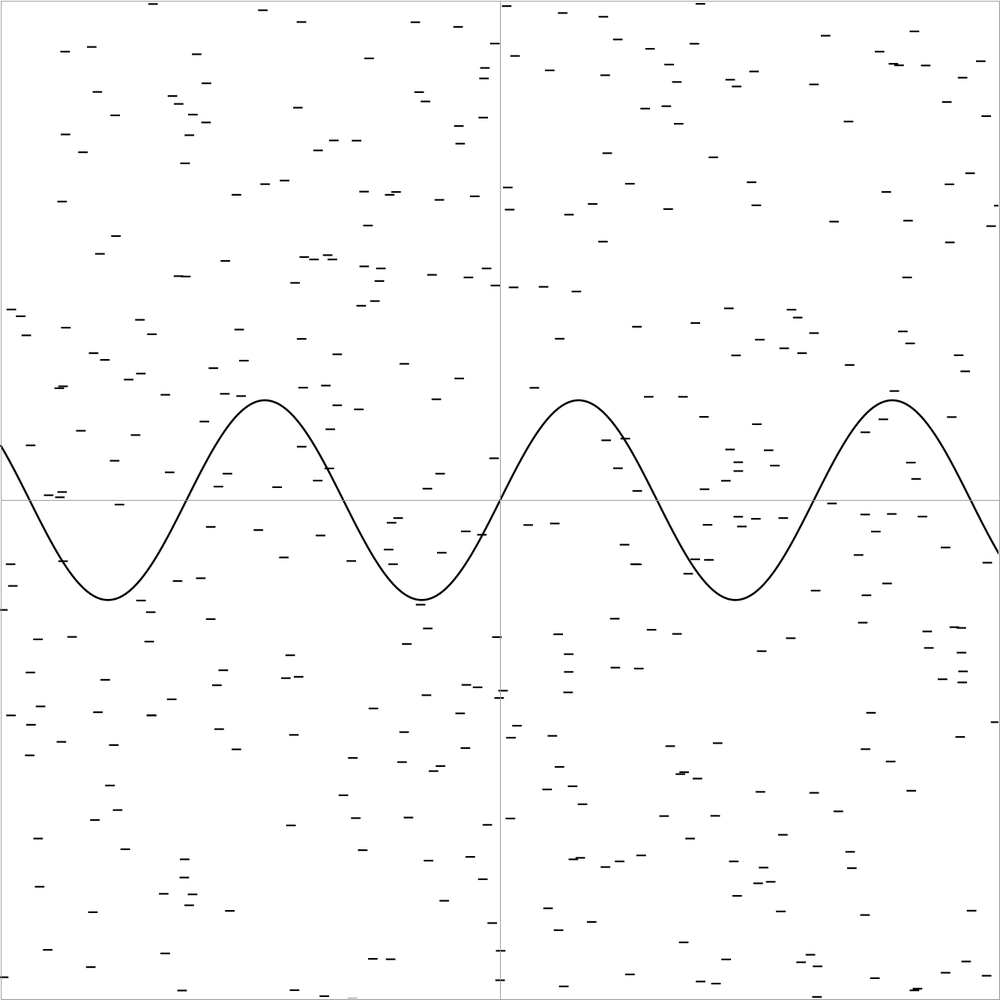
\includegraphics[width=\textwidth]{primer1_1}
		\caption{График неточного решения}
		\label{image1}
	\end{subfigure}
	\hfill
	\begin{subfigure}[b]{0.45\textwidth}
		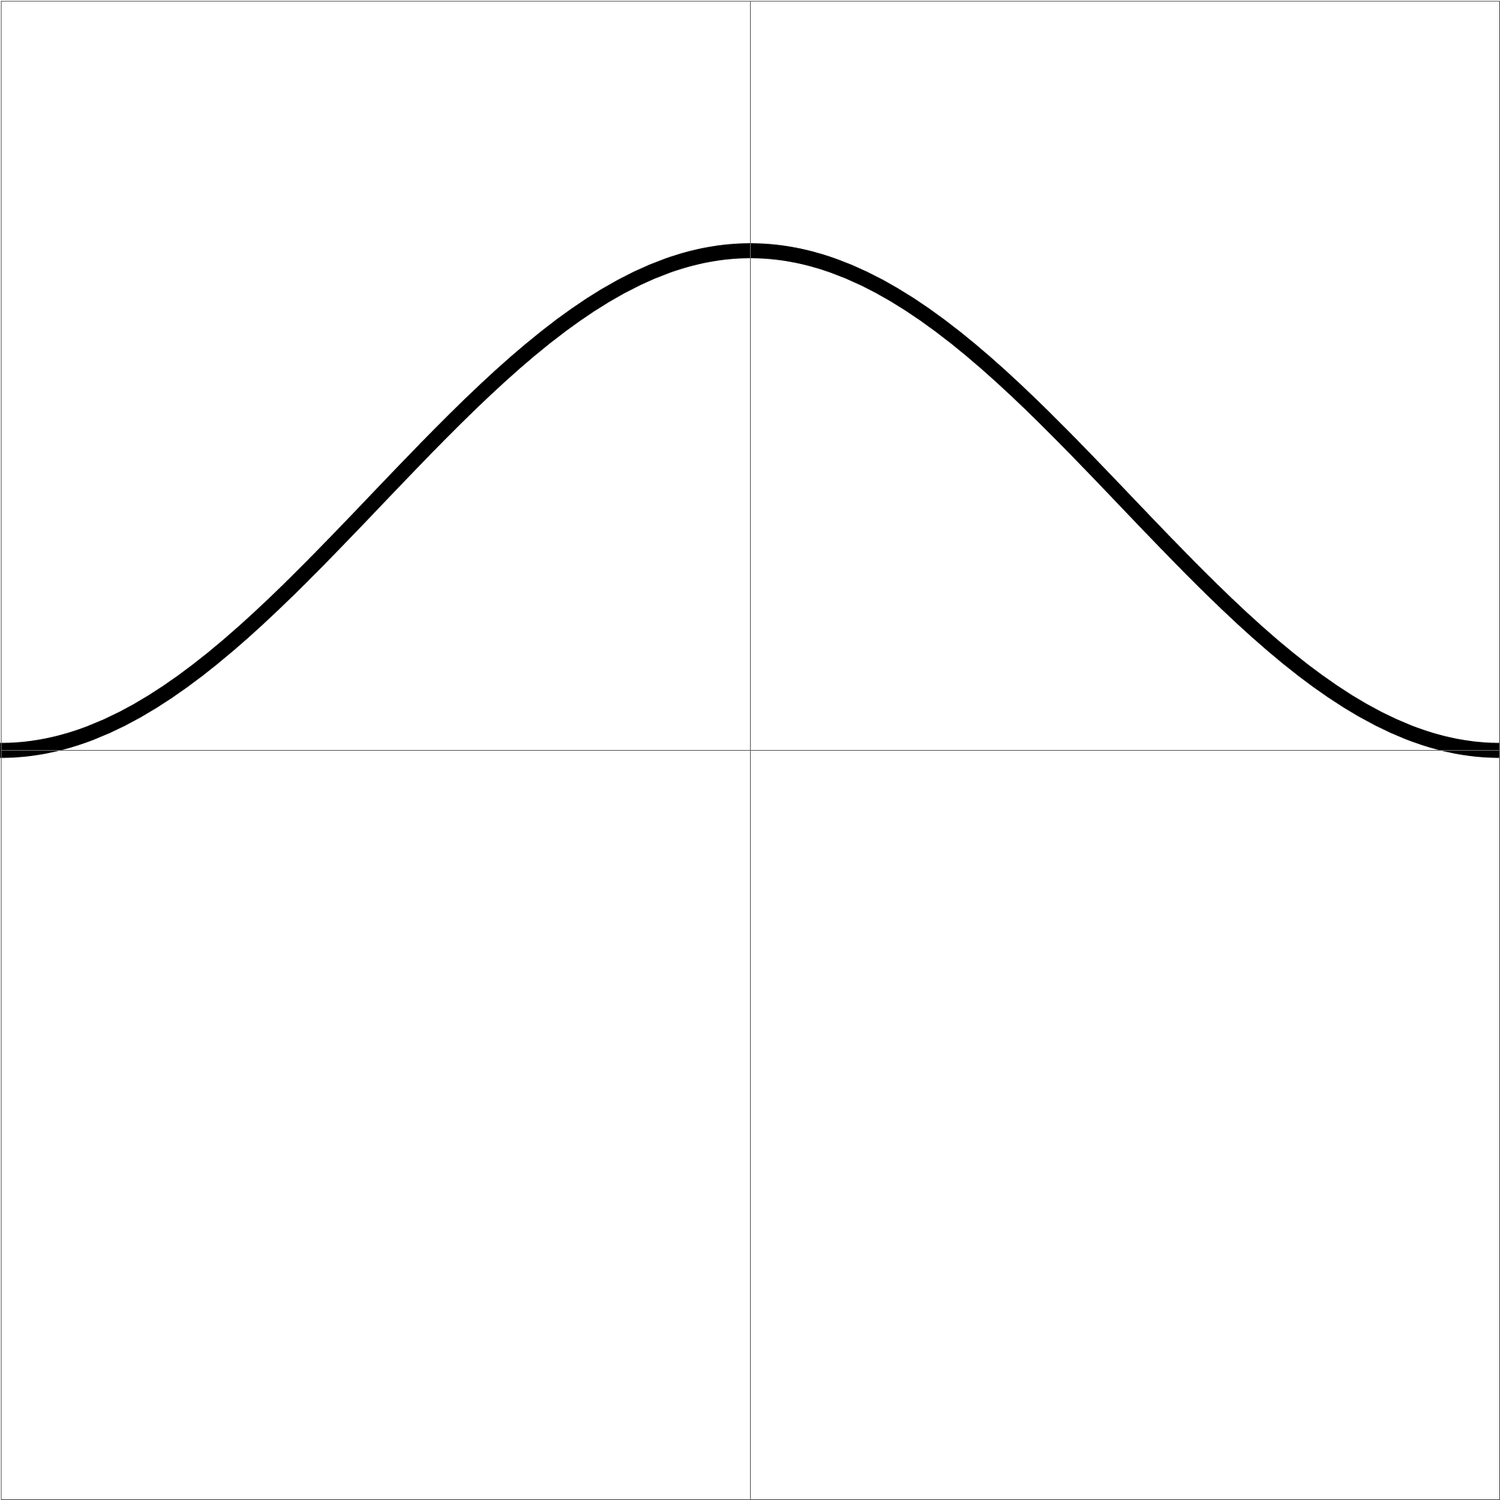
\includegraphics[width=\textwidth]{test4}
		\caption{График точного решения}
		\label{image2}
	\end{subfigure}
	\caption{Иллюстрация задачи}
\end{figure}

К поставленной задаче, в силу свойств выбранного метода решения, ставятся некоторые ограничения. График будем рассматривать только в определенной области, а все возможные решения будем считать известными и их количество ограниченным. Тем самым, будем рассматривать только определенные наборы решений в выбранные моменты времени на некотором интервале.

\section{Задача Коши для линейного одномерного уравнения переноса}
Уравнение переноса является одним из фундаментальных уравнений математической физики, которое широко используется для описания движения сплошной среды. В то же время оно является простейшим представителем семейства гиперболических уравнений, которые определяются наличием действительных характеристик, число которых совпадает с числом неизвестных для системы уравнений первого порядка. Рассмотрим задачу Коши для уравнения переноса следующего вида:
\begin{equation}
	\begin{cases}
		\dfrac{\partial u}{\partial t} + a\dfrac{\partial (u)}{\partial x} = 0, \\
		u(x, 0) = u_0(x),
	\end{cases} 
	\text{где } u = u(x, t), \quad a = const > 0, \quad t \in (0, T), \quad x \in (-\infty, +\infty) .
\end{equation}


Приведем аналитическое решение. Уравнение можно записать в виде:
\begin{equation*}
	u_t + a u_x = 0
\end{equation*}
Запишем и решим характеристическое уравнение:
\begin{equation*}
	\dfrac{dt}{1} = \dfrac{dx}{a} = \dfrac{du}{0} \quad \implies  \quad 
	\begin{cases}
		u = C_1,\\
		x = a t + C_2
	\end{cases} 
	\quad \implies \quad
	\begin{cases}
		C_1 = u,\\
		C_2 = x - at
	\end{cases}
	 \quad \implies \quad
	 u = \psi(x-a t).
\end{equation*}
Применим граничные условия:
\begin{equation*}
	u(x, 0) = u_0(x),
	\quad \implies \quad
	\psi(x) = u_0(x),
	 \quad \implies \quad
	 u = u_0(x-a t).
\end{equation*}
Получим аналитическое решение уравнения $u = u_0(x-at)$. Решение заключается в сносе неизменного профиля по характеристикам. 

Важнейшим свойством рассматриваемого решения будет являться сохранение начального профиля: если начальное решение представляет собой, например, профиль буквы «М», то оно будет сохранять его таким всегда.

\section{Численные методы решения задачи}
Целью построения методов численного решения данного уравнения является не собственно нахождение его решения, а исследование численного алгоритма на простейшем примере. Аналитическое решение данного уравнения известно и тривиально. При этом в чрезвычайно большое количество математических моделей уравнение переноса входит в качестве составной части. К таким относятся модели газодинамики, гидродинамики, переноса частиц и излучения, электродинамики и многие другие. Разработать метод численного решения для этих моделей можно только в том случае, если метод будет построен и успешно применен для данного простейшего уравнения, описывающего обыкновенный перенос.\cite{1}
\subsection{Описание методов}
Обозначим $\gamma =  \dfrac{a \tau}{h}$ --- число Куранта. Для численного решения задачи Коши для линейного одномерного уравнения переноса рассмотрим следующие схемы:



\begin{enumerate}

	\item \textbf{Явная схема с левой разностью по двум точкам}:
	\begin{equation*}
		\widehat{y} = (1 - \gamma) y + \gamma y_{-1}.
		\label{s1}
я	\end{equation*}
	
	Погрешность аппроксимации схемы: 
	$\psi_h = O(\tau + h)$.
	
	Схема устойчива при $\gamma \leq 1 $, причем при $\gamma = 1$ схема является точной.
	
	\bigskip
	\item \textbf{Неявная схема с левой разностью по двум точкам}:
	\begin{equation*}
		\widehat{y} = \dfrac{\gamma}{1 + \gamma} \widehat{y}_{-1} + \dfrac{1}{1 + \gamma} y .
		\label{s2}
	\end{equation*}
	
	Погрешность аппроксимации схемы: $\psi_h = O(\tau + h)$.
	
	Данная схема является безусловно устойчивой.
	
	\bigskip
	\item \textbf{Явная схема с левой разностью по трем точкам}:
	\begin{equation*}
		\widehat{y} = (1 - \frac{3}{2}\gamma) y + \gamma(2y_{-1} - \frac{1}{2}y_{-2}).
		\label{s3}
	\end{equation*}
	
	Погрешность аппроксимации схемы: 
	$\psi_h = O(\tau + h^2)$.
	
	Схема является безусловно неустойчивой.
	
	\bigskip
	\item \textbf{Неявная схема с левой разностью по трем точкам}:
	
	\begin{equation*}
		\widehat{y} = y - \gamma (\widehat{y}_{-1} - \widehat{y}_{-2})
		\label{s4}
	\end{equation*}
	Погрешность аппроксимации схемы: $\psi_h = O(\tau + h)$.
	Схема является безусловно неустойчивой.
	
	\item \textbf{Схема Лакса}:
	\bigskip
	\begin{equation*}
		\widehat{y} = \dfrac{(y_{+1} + y_{-1}) - \gamma(y_{+1} - y_{-1})}{2} .
		\label{s5}
	\end{equation*}
	
	Погрешность аппроксимации схемы: $\psi_h = O(\tau + h + \frac{h^2 }{ \tau})$.
	
	Схема устойчива при $\gamma \leq 1 $ и сходится при стремлении $h^2 \to 0$ быстрее, чем $\tau$.
	\bigskip
	\item \textbf{Схема Лакса-Вендрофа}:
	\begin{equation*}
		\widehat{y} = y - \gamma(\dfrac{(y_{+1} + y) - \gamma (y_{+1} - y)}{2} -  \dfrac{(y + y_{-1}) - \gamma (y - y_{-1})}{2}).
		\label{s6}
	\end{equation*}
	
	Погрешность аппроксимации схемы: 
	$\psi_h = O(\tau^2 + h^2)$.
	
	Схема устойчива при $\gamma \leq 1 $, а при $\gamma = 1$ схема является точной. 
	
\end{enumerate}

\subsection{Реализация}

Все эти схемы реализованы в программе на языке программирования C++. Был создан единый программный класс, который включает в себя все необходимые данные об уравнении и методе, а также сами реализации методов. Программа возвращает массив с результатами, записанный в текстовый файл.


Для тестирования были взяты следующие начальные условия:
\begin{figure}[!hp]
	\centering
	\begin{subfigure}[t]{0.32\textwidth}
		\centering
		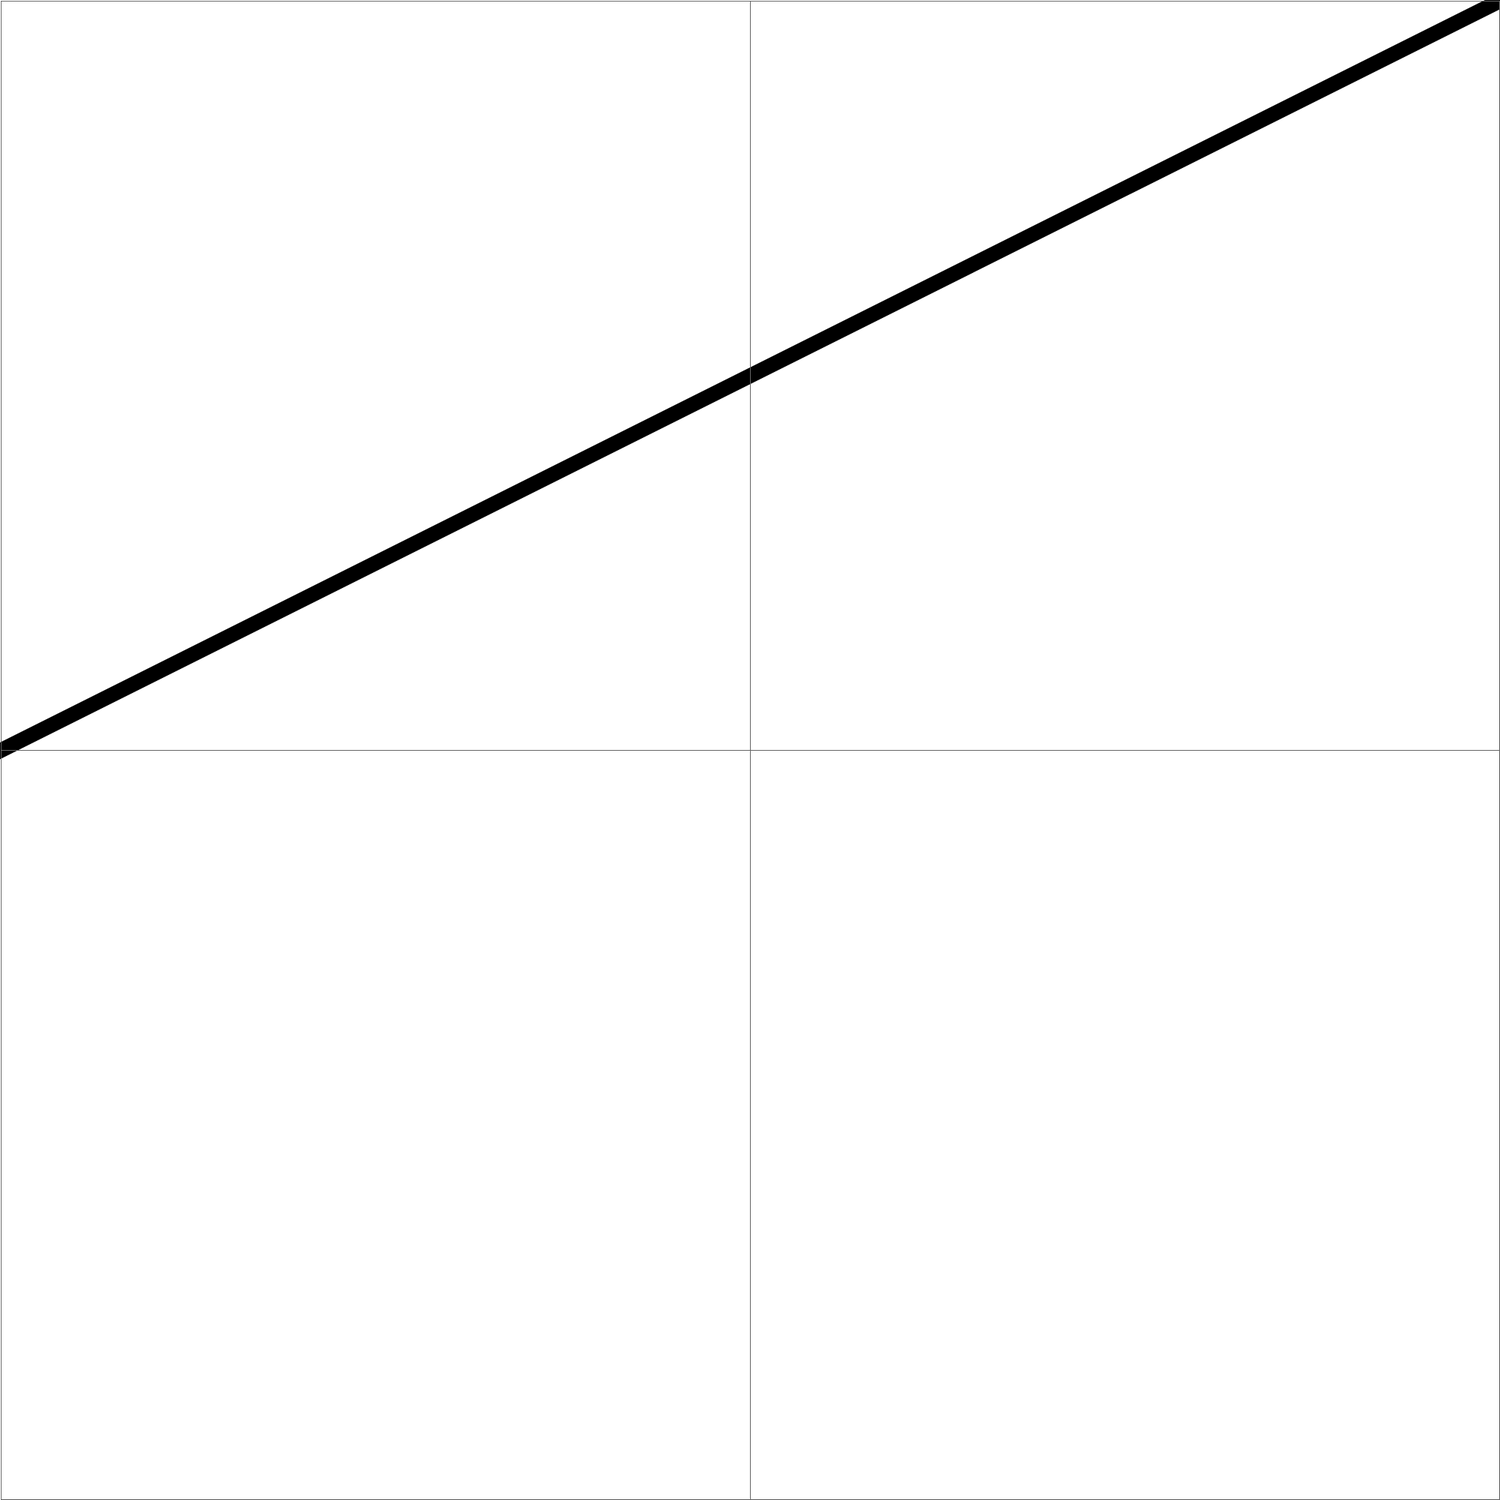
\includegraphics[width=\textwidth]{test1}
		\caption{Левый треугольник \\ $u_0 = \frac{x-l_1}{l_2-l_1}$}
		\label{test1}
	\end{subfigure}
	\hfill
	\begin{subfigure}[t]{0.32\textwidth}
		\centering
		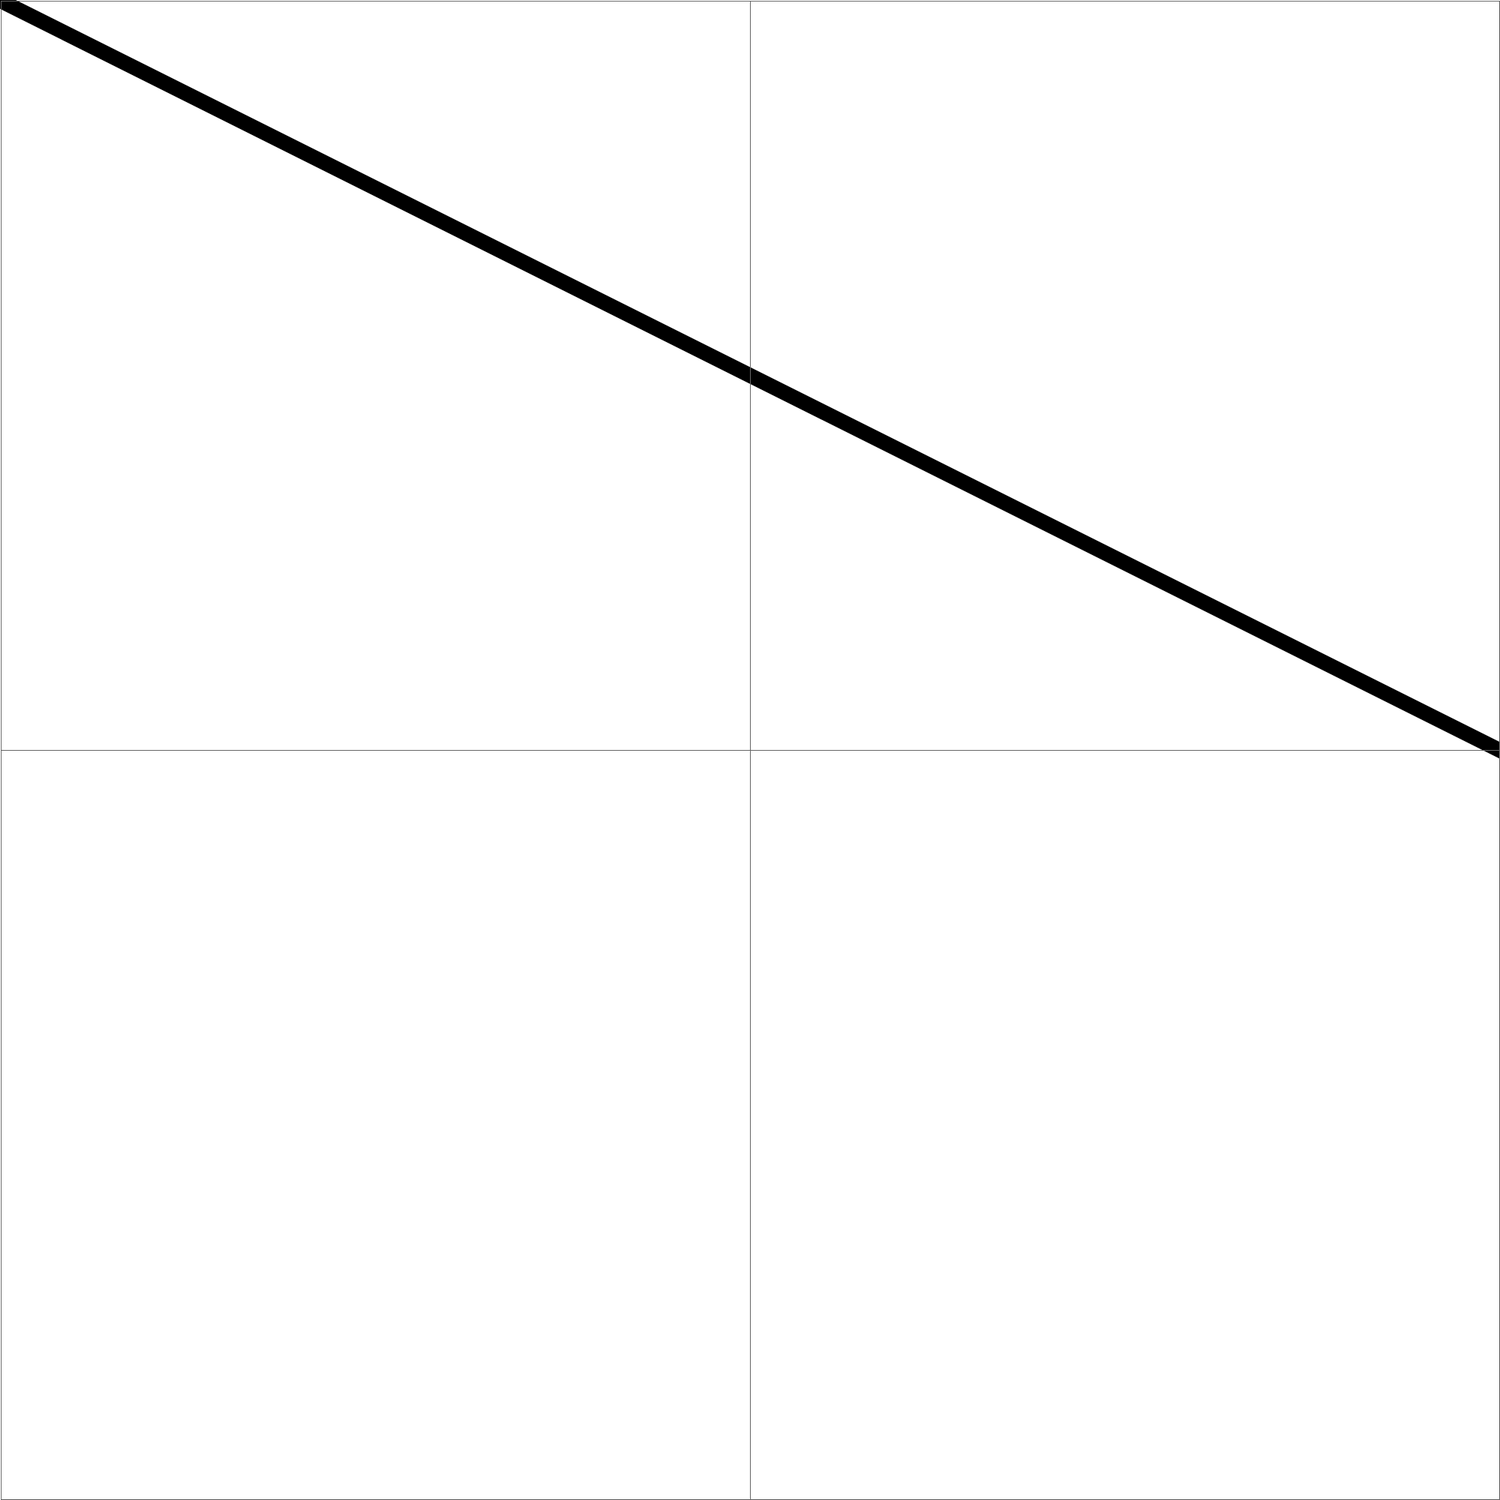
\includegraphics[width=\textwidth]{test2}
		\caption{Правый треугольник \\ $u_0 = \frac{l_2-x}{l_2-l_1}$}
		\label{test2}
	\end{subfigure}
	\hfill
	\begin{subfigure}[t]{0.32\textwidth}
		\centering
		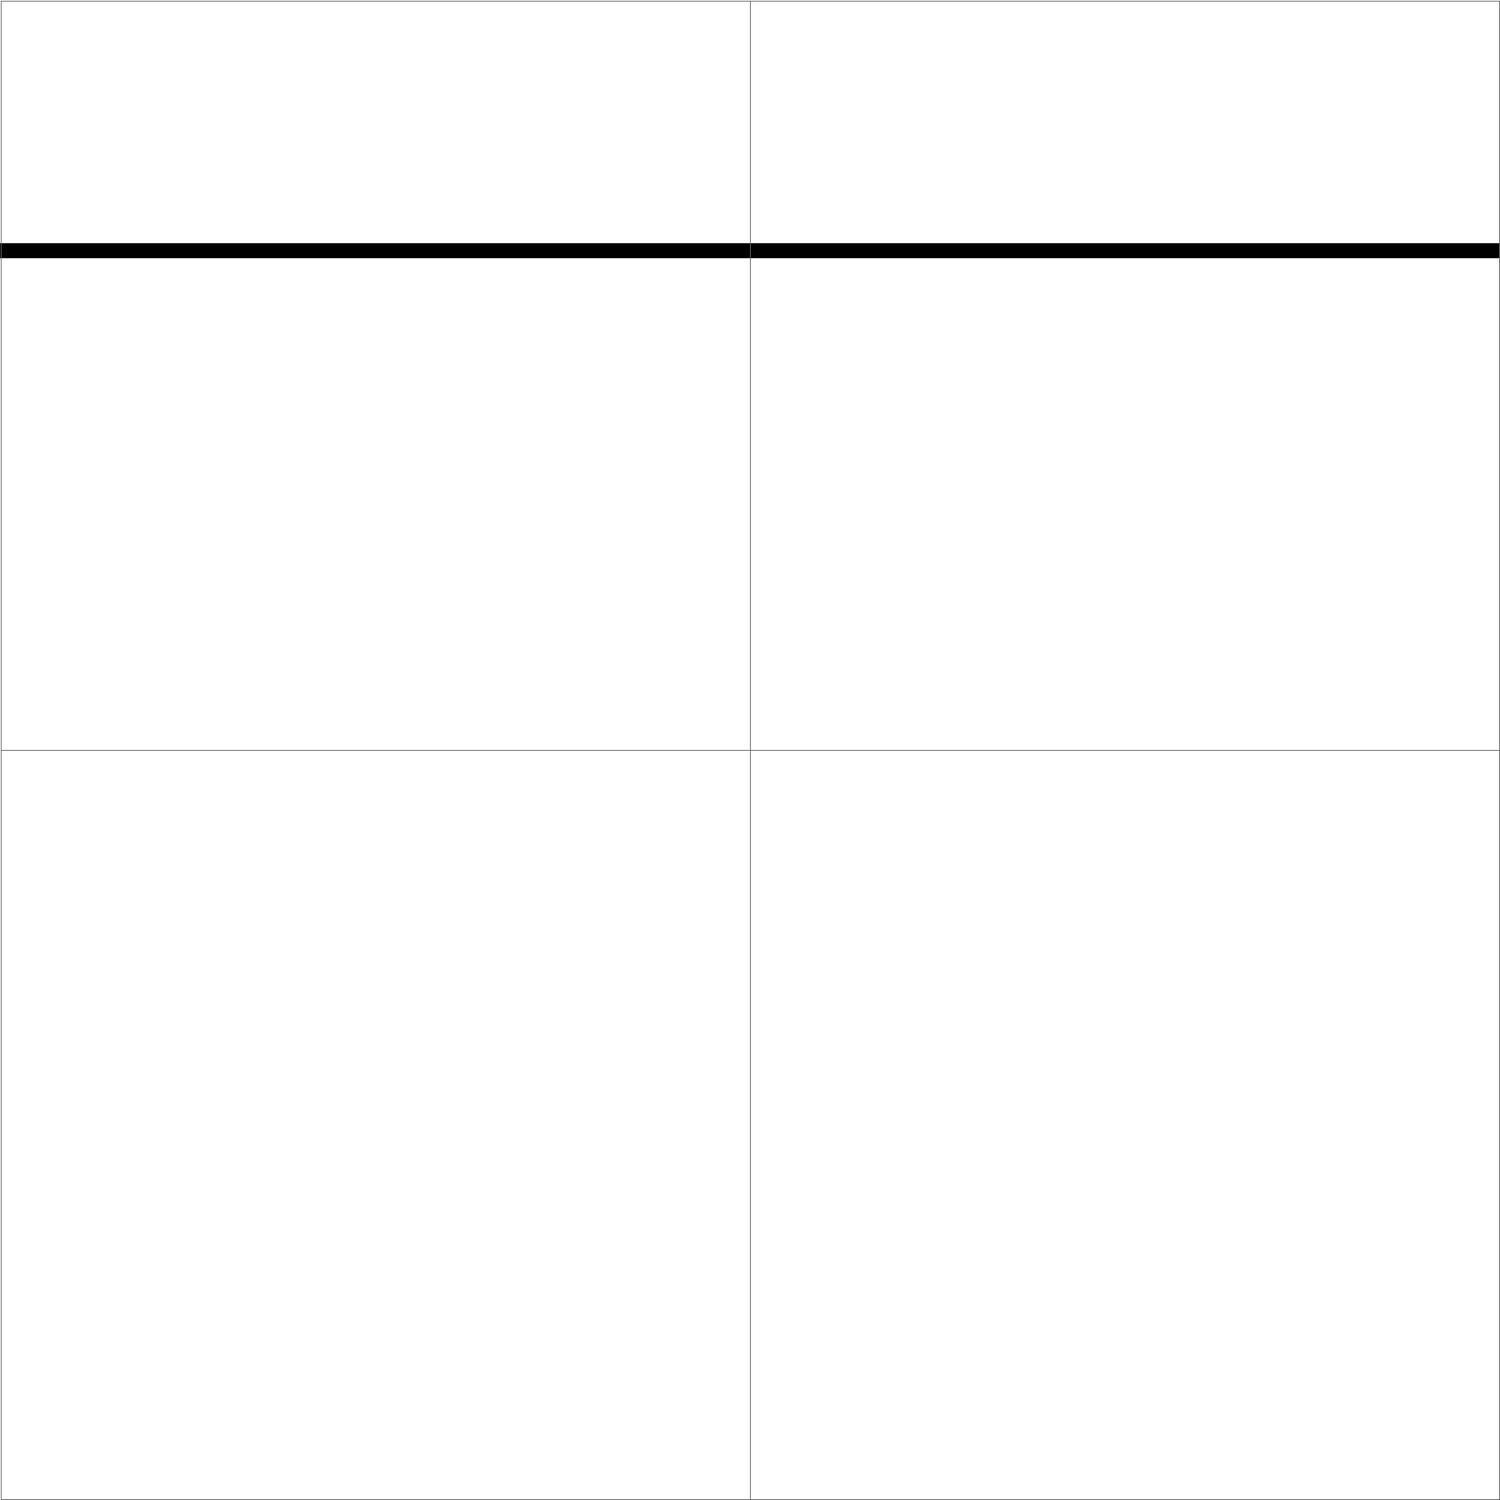
\includegraphics[width=\textwidth]{test3}
		\caption{Прямоугольник \\ $u_0 = \frac{2}{3}$}
		\label{test3}
	\end{subfigure}
	
	\vspace{1em}
	
	\begin{subfigure}[t]{0.475\textwidth}
		\centering
		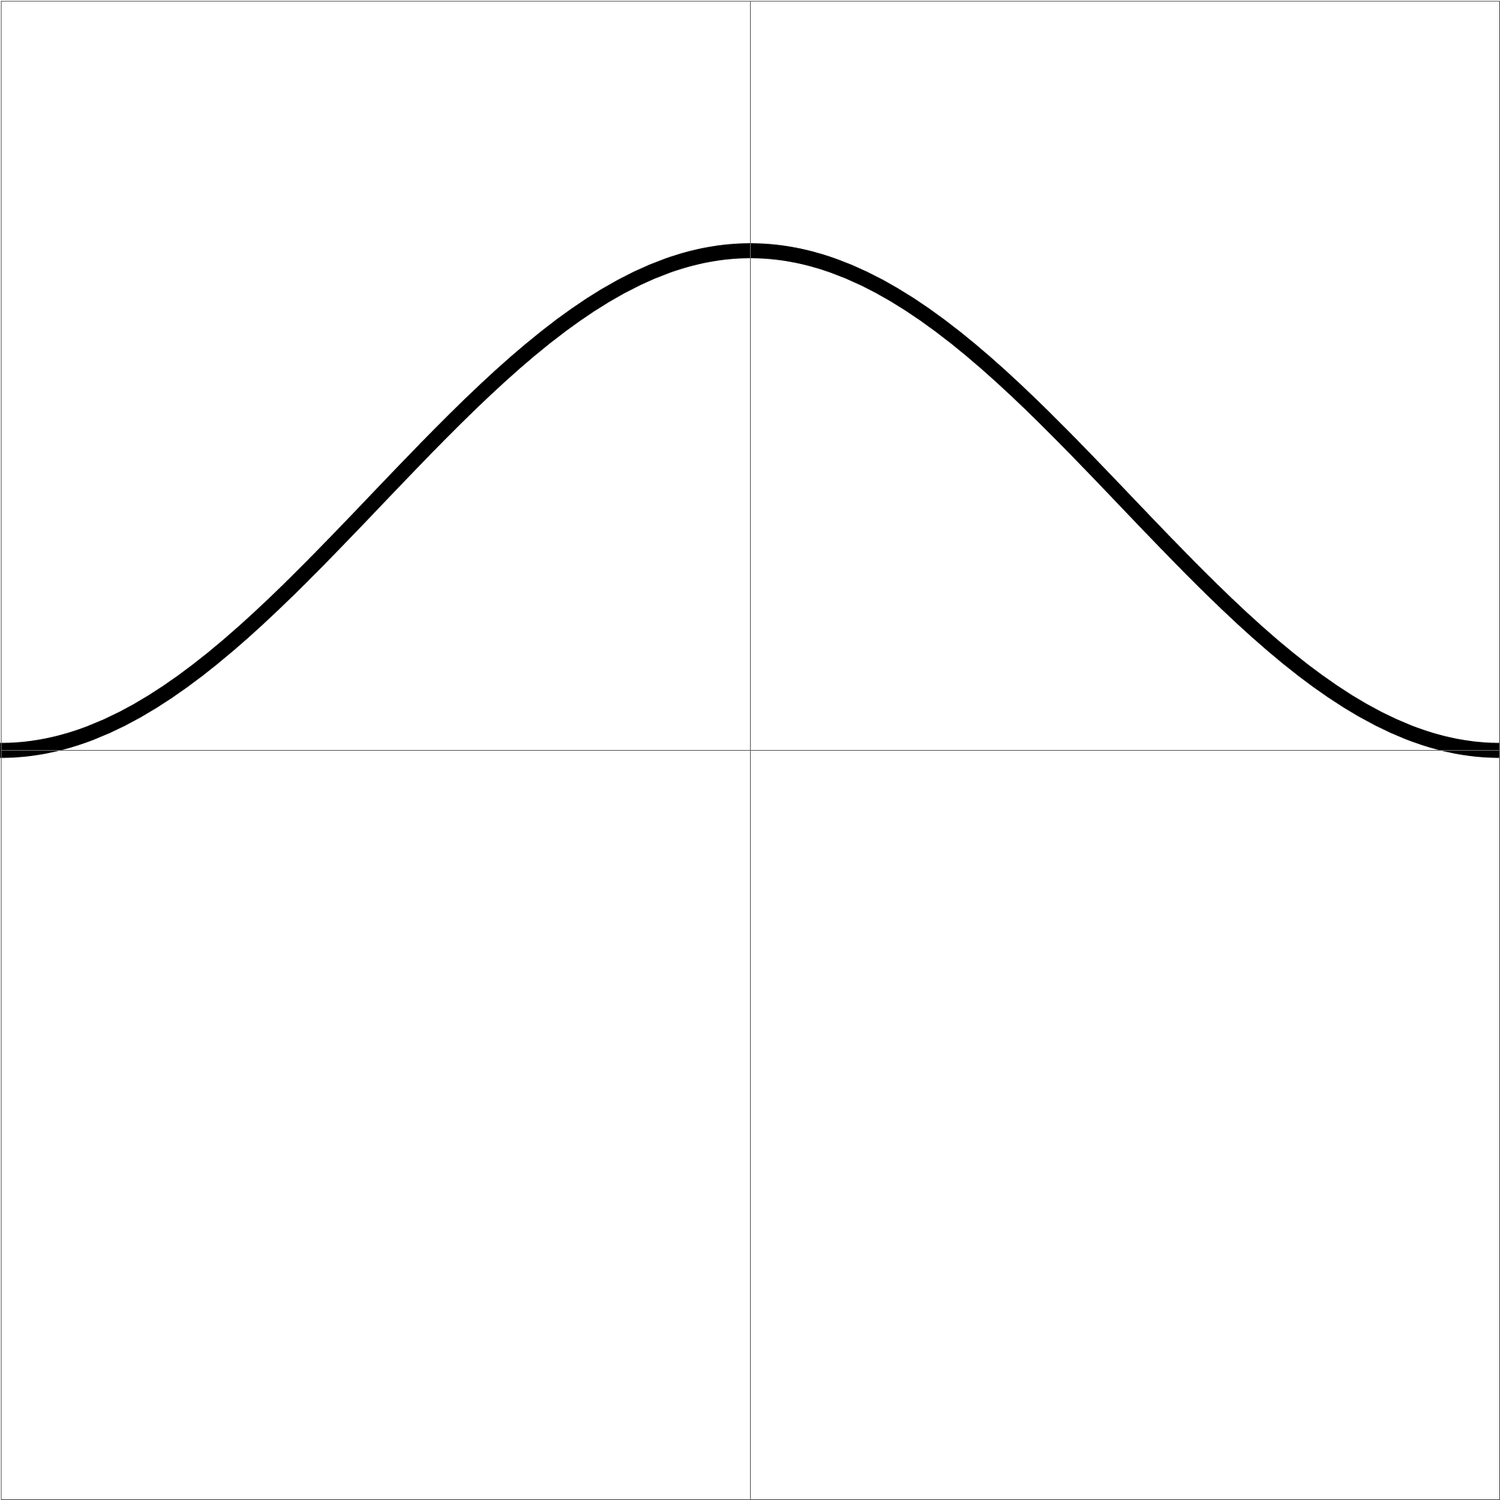
\includegraphics[width=\textwidth]{test4}
		\caption{Косинус \\ $u_0 = \frac{1}{3} (1 - \cos(\frac{2 \pi (x - l_1)}{l_2 - l_1}))$}
		\label{test4}
	\end{subfigure}
	\hfill
	\begin{subfigure}[t]{0.475\textwidth}
		\centering
		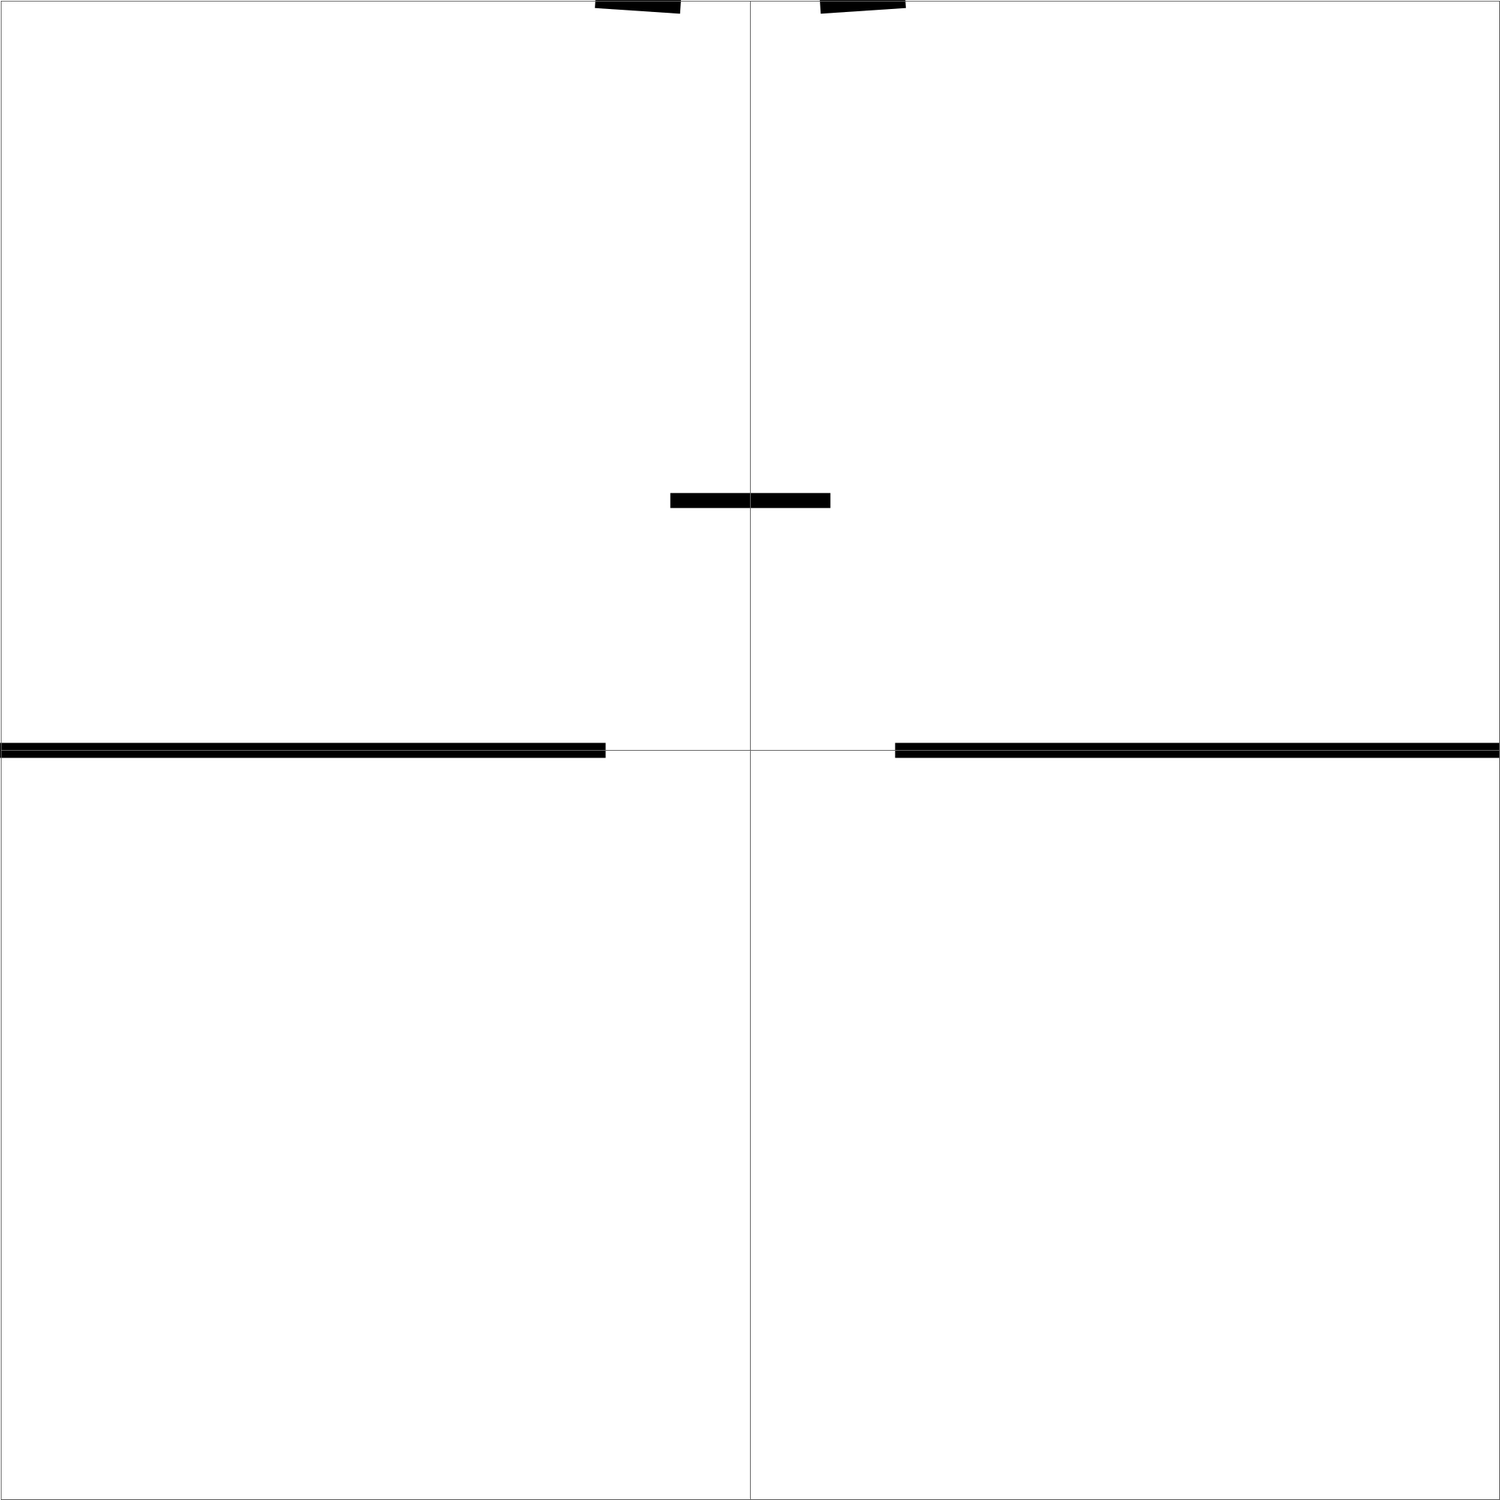
\includegraphics[width=\textwidth]{test5}
		\captionsetup{singlelinecheck=off}
		\caption[]{«Зуб»
			\[
			\hspace*{-0.75cm}u_0(x) =
			\begin{cases}
				-\frac{2}{3} (l_{11} - l_1) (x - l_1) + 1, & l_1 \leq x < l_{11} \\
				\frac{1}{3}, & l_{11} \leq x \leq l_{22} \\
				\frac{2}{3} (l_2 - l_{22}) (x - l_2) + 1, & l_{22} < x \leq l_2
			\end{cases}
			\]
		}
		\label{test5}
	\end{subfigure}
\end{figure}

 Для расчета по схемам организован итерационный процесс. Первой итерацией в объект std::vector записывается начальное условие. На каждом шаге по времени записывается новый вектор значений, который изменяется в соответствии со схемой. Для явных схем процесс организован в виде последовательного вычисления верхнего слоя значений исходя из нижнего. В случае неявных схем (\ref{s2}) и (\ref{s4}) задается левое граничное условие, которое является аналитическим решением соответствующего теста в точке левой границы. Процесс схемы (\ref{s2}) дальше выполняется также как и по явной схеме, а в схеме (\ref{s4}) на каждом шаге решается система алгебраических уравнений методом прогонки.
 
Покажем сходимость или расходимость схем путем вычисления нормы ошибки.

\begin{table}[ht!]
	\caption{Нормы ошибки разностных схем}
	\centering
	\begin{tabular}{|l|l|l|l|}
		\hline
		\diagbox{$h, \tau$}{Схема}       & Явная ЛДР 1-го пор.     & Неявная ЛДР 1-го пор.  & Явная ЛДР 2-го пор.    \\ \hline
		\textbf{$h = 0.1, \tau = 0.1$}   & $ 4.44 \cdot 10^{-16}$  & $ 4.2 \cdot 10^{-2}$ &  $1632$   \\ \hline
		\textbf{$h = 0.05, \tau = 0.1$}  & $5.2 \cdot 10^{-3} $      & $6.7 \cdot 10^{-3} $ &  $1229$ \\ \hline
		\hline
		\diagbox{$h, \tau$}{Схема}       & Неявная ЛДР 2-го пор.   & Лакса                  & Лакса-Вендрофа          \\ \hline
		\textbf{$h = 0.1, \tau = 0.1$}   & $10^{18}$               & $9.1 \cdot 10^{-2} $   & $4.46 \cdot 10^{-16} $  \\ \hline
		\textbf{$h = 0.05, \tau = 0.1$}  & $10^{54}$               & $3.3 \cdot 10^{-6} $  	& $5.4 \cdot 10^{-6} $    \\ \hline
	\end{tabular}
	\label{tab1}
\end{table}
Норма вычислялась как максимум разности численного и аналитического решений в точках сетки. Вычисления проводились на тесте «левый треугольник». Сетка строилась до момента времени $T = 3$.

Результаты в таблице \ref{tab1} дают подтверждение, что схемы (\ref{s3}) и (\ref{s4}) расходятся при любых параметрах, схемы (\ref{s1}) и (\ref{s6}) точны при $\gamma = 1$.

 Для визуализации решения использовался математический пакет Wolfram Mathematica, в котором были созданы функции для создания анимации изменения графика во времени. Также в этом пакете были созданы функции для визуализации аналитического решения и для сравнения его с численным.

\clearpage
\section{Метод улучшения решения с помощью нейронной сети}

Основной целью данной работы является создание программы, которая по известному точному решению сможет улучшить входное неточное. Для реализации такой программы был выбран метод, заключающийся в распознавании изображения нейронной сетью. Алгоритм модели заключается в следующем: в сеть, обученную на исключительно точных решениях, подается на вход неточное, которое она классифицирует. Как результат, нейросеть выдает метку соответствующего точного решения.

\subsection{Модель сверточной нейронной сети}

Сверточная нейронная сеть - модель нейронной сети, предложенная в 1988 году Яном Лекуном, которая и сегодня является одной из самых эффективных для распознавания образов на изображении. Структура сети однонаправленная и для обучения в большинстве случаев используется метод обратного распространения ошибки. \cite{2}

Основной особенностью сверточной нейронной сети является наличие комбинаций слоев свертки и пуллинга. Преимущества модели, заключается в способности улавливать пространственные взаимосвязи на изображении, что позволяет классифицировать одни и те же объекты независимо от их расположения и размера на изображении. Не менее значимым является меньшее количество настраиваемых весов, так как один набор фильтров как весы используется целиком для всего изображения, вместо того, чтобы создавать для каждого пикселя входного изображения свои коэффициенты как это делает перцептрон. Благодаря такой особенности, сверточная нейронная сеть требует меньшее количество времени для обучения. Также данная модель устойчива к повороту и сдвигу распознаваемого изображения. 

Для реализации своей модели выберем библиотеку $TensorFlow$ в силу ее простоты и полноты документации. Опишем основные шаги при создании модели сверточной нейросети с помощью библиотеки TensorFlow. 

 Модель нейросети представляет собой объект класса из TensorFlow, который мы назовем $Model$. При создании модели необходимо указать ее тип как $sequental$, что означает, что процесс вычислений будет последовательно идти по слоям. После создания модели необходимо добавить в нее слои, что можно сделать с помощью метода $.add$. Добавляя нужное нам количество уже встроенных в библиотеку слоев свертки $Conv2D$, указываем количество фильтров, их размерность и функцию активации. Добавляем слои пуллинга $MaxPooling2D$, указывая в параметрах слоя необходимую размерность подвыборки. Последними слоями будут полносвязные слои $Dense$, где указываем количество нейронов и также функцию активации. Количество вариантов ответа нейросети обозначим $output$.
 
  Наконец, соберем модель с помощью метода $.compile$, в котором необходимо указать параметры функции оптимизатора, потерь и метрику обучения.  Для использования модели остается только ее скомпилировать с помощью метода $.compile$. 
 
 Библиотека позволяет сохранить параметры скомпилированной модели, что делает возможным встраивать уже созданный алгоритм распознавания в другие программы. Таким образом можно создать свою модель нейронной сети для совершенно разных задач.
 
  \lstinputlisting[caption={Модель нейронной сети}, inputencoding=utf8]{code/Model.py}
 
 
\subsection{Распознавание решения}

Чтобы распознать на изображении определенное решение уравнения, необходимо произвести расчет модели нейронной сети и получить ее ответ. Этим ответом будет метка, которая была назначена во время обучения каждому решению. Зная метку, можно поставить в соответствие исходное для обучения изображение, которое и будет являться улучшенным решением. 

Для работы такого подхода была реализована программа на языке программирования Python, которая включает в себя все прежде описанные действия. На вход программа получает изображение (путь к изображению в операционной системе), которое она преобразовывает в объект, который можно подать в модель нейронной сети для получения предсказания метки. Программа вызывает заранее обученную нами модель нейронной сети и получает ее ответ. При обучении модели автоматически создается кодификатор, который ставит соответствие между каждой меткой и изображении, на котором производилось обучение. Программа использует этот кодификатор и возвращает тем самым изображение, которое является точным решением.

\subsection{Результаты работы программы}
Для проверки работы программы был созданы наборы изображений для обучения и тестирования. Наборы содержали решения для промежутка времени $t \in [0, 1]$ с шагом $0.1$. Рассматривалась область $x \in [-1, 1], y \in [-1, 1]$, а изображения составлялось разрешением в $128 \cdot 128$ пикселей. Для теста использовались решения, полученные с помощью определенных схем, которые решают уравнение хотя бы примерно. 

Приведем таблицу результатов точности работы программы в зависимости от шагов по времени и пространству.

\begin{table}[ht!]
	\caption{Результаты тестирования модели нейронной сети}
	\centering
	\begin{tabular}{|l|l|l|l|}
		\hline
		Номер теста & Шаг по времени $\tau$  & Шаг по пространству $h$ & Точность программы \%      \\ \hline
		\textbf{1}  & 0.1                    & 0.1    				   & 82          				\\ \hline
		\textbf{2}  & 0.05                    & 0.1   			       & 84         				\\ \hline
		\textbf{3}  & 0.05                   & 0.05   				   & 89        			    \\ \hline
		\textbf{4}  & 0.01     `			 & 0.01  				   & 93     					\\ \hline
	\end{tabular}
\end{table}

Стоит отметить, что результаты могут отличатся в зависимости от множества факторов, к которым относятся выбор коэффициентов сети, количество эпох обучения и особенности выбора набора для обучения.

\section{Актуальность и перспективы задачи}
Технологии нейронных сетей пробираются во все сферы деятельности человека и применение их в математике может привести к неожиданно полезным результатам. Благодаря распознаванию графика функции нейронной сетью, можно научить компьютер определять одновременно огромное количество графиков за сравнено небольшое количество времени, чтобы применять данный метод в совершенно разных сферах науки и техники. Перспективой развития данного метода является создания такого же алгоритма восстановления графика решений, но с заранее неизвестными данными о типе графика. Улучшение распознавания типов графиков приведет к возможностям классифицировать практически любое решение уравнения и уточнить его на любом малом промежутке исходную кривую.

\section-{Заключение}
Таким образом в ходе работы были изучены численные методы решения уравнения переноса, проведено тестирование численных методов на 5 тестах, а также созданы несколько программ. Была создана программа, которая по неточному решения уравнения переноса возвращает точное. Была реализована программа на языке программирования С++17 для численного решения уравнения переноса различными схемами, а также реализованы 5 тестов. Реализована модель сверточной нейронной сети для распознавания решений уравнения на языке программирования Python 3.9.2 с помощью библиотеки машинного обучения TensorFlow 2.15.0. Изображения графиков решения создавались с помощью математического пакета Wolfram Mathematica 14. c реализацией соответствующих функций. 

Как итог, реализована программа, которая с помощью модели сети улучшает неточное решение данного уравнения до точного.  
 


\clearpage
\begin{thebibliography}{1}

\bibitem{1} Галанин М.П., Савенков Е.Б. Методы численного анализа математических моделей. М.: Изд-во МГТУ им. Н.Э. Баумана. 2018. 592 с.


\bibitem{2} Tariq Rashid Make Your Own Neural Network // CreateSpace Independent Publishing Platform; 1st edition SAND96-0583 (March 31, 2016)


\bibitem{3} TensorFlow documentation. URL: https://www.tensorflow.org/?hl=ru (Дата обращения 08.06.2024)

%\bibitem{5} Keras documentation URL: https://keras.io (Дата обращения 17.01.2024)

\bibitem{4} Гафаров Ф.М. Искусственные нейронные сети и приложения. г.Казань: Изд-во Казан. ун-та, 2018. 121 с


\end{thebibliography}

\end{document} 